\subsubsection{Descripción}

Un algoritmo goloso usa una heur\'istica que consiste en elegir, en cada paso, una soluci\'on \'optima local entre un conjunto de opciones, esperando encontrar al final la soluci\'on \'optima global. En general estos algoritmos son eficientes y simples de dise\~nar e implementar, pero puede ser que nunca lleguen a la soluci\'on \'optima del problema. 

De acuerdo a la definici\'on de Brassard\footnote{\label{Brassard}Brassard G., Bratley P., {\it Fundamental of Algorithmics}, Prentice Hall, 1996. (c)}, un algoritmo goloso se compone de los siguientes elementos: 

\begin{enumerate}
 \item Un concepto de candidato, y una estructura de solución a partir de candidatos.
 \item Un conjunto de candidatos que ya han sido considerados y seleccionados. 
 \item Un conjunto de candidatos considerados y rechazados. 
 \item Una funci\'on que comprueba si cierto conjunto de candidatos constituye una soluci\'on a nuestro problema, ignorando si es o no \'optima por el momento. 
 \item Una funci\'on de factibilidad, que determina si es o no posible completar el conjunto a\~nadiendo otros candidatos para obtener al menos una soluci\'on de nuestro problema. 
 \item Una funci\'on selecci\'on que indica en cualquier momento cu\'al es el m\'as prometedor de los candidatos restantes, que no han sido seleccionados ni rechazados. 
 \item Una funci\'on objetivo, que da el valor de la soluci\'on que hemos hallado. 
\end{enumerate}

Lo que busca el algoritmo goloso es encontrar la secuencia de candidatos que constituya una soluci\'on, y que optimice el valor de la funci\'on objetivo. Este algoritmo avanza paso a paso. Inicialmente, el conjunto de elementos seleccionados est\'a vac\'io. Entonces, en cada paso se considera a\~nadir a este conjunto el mejor candidato sin coniderar los restantes, de acuerdo a nuestra funci\'on selecci\'on. Si el conjunto ampliado de candidato seleccionados ya no fuera factible, rechazamo el candidato que estamos considerando en ese momento. Sin embargo, si el conjunto aumentado sigue siendo factible, entonces a\~nadimos el candidato actual al conjunto de candidatos selecccionados, en donde pasar\'a a estar desde ahora en adelante. Cada vez que se ampl\'ia el conjunto de candidatos seleccionados, comprobamos si \'este constituye ahora una soluci\'on para nuestro problema. A partir de este esquema, al agregar siempre subsoluciones \'optimas a mi conjunto, al finalizar lo que se espera encontrar es la soluci\'
on \'optima. 

El algoritmo de Dijsktra para encontrar caminos m\'inimos en un grafo pesado es un algoritmo goloso, que funciona y es correcto, como lo fue demostrado por Bassard en el libro mencionado.

Dado un grafo $G=(V,X)$, Dijkstra guarda un conjunto $S$ de nodos que ya fueron recorridos y un vector $\pi$ con la distancia m\'inima de un nodo $u$ a todos los de $S$. En cada fase de Dijkstra, se selecciona un nuevo nodo de $V\backslash S$ cuyo valor en $\pi$ sea m\'inima y lo a\~nadimo a $S$, actualizando si es necesario $\pi$. Al finalizar, $\pi$ es el vector con la m\'inima distancia a todos los nodos. 

Entonces, nosotros para resolver el problema vamos implementar Dijkstra con tres funciones objetivo diferentes, que toman una arista y devuelven un peso para ella: 

\begin{enumerate}
  \item $f_A(e) = \omega_1(e)$
  \item $f_B(e) = \omega_2(e)$
  \item $f_C(e) = \omega_1(e)\omega_2(e)$
\end{enumerate}

Luego el pseudoc\'odigo de Dijkstra modificado con la nueva definici\'on de distancia queda dado por: 

\begin{algorithm}
In: Grafo $G = (V,X)$, nodo inicial $v_0$, ObjectiveFunction $f$ \newline
Out: Arreglo $\pi$ con camino m\'inimo en funci\'on de $f$ a cada nodo. 
\begin{algorithmic}[1]
\State $\pi(v) = \infty$ \quad $\forall v \in V$
\State $\pi(v_0) = 0$
\State $S = \emptyset$
\For{$i = 1 \dots n-1$}
    \State $v \leftarrow $ nodo de $V\backslash S$ de m\'inimo $\pi$. 
    \For{{\bf each} $w \in V\backslash S$ adyacente a $v$}
      \State $\pi(w) = \min( \pi(w), \pi(v) + f((v,w)))$
    \EndFor
    \State $S = S \cup \{v\}$
\EndFor
\State \textbf{retornar} $\pi$
\end{algorithmic}
\end{algorithm}

La modificaci\'on est\'a la l\'inea 7, que en vez de sumar a $\pi(v)$ el peso de la arista, como es en el algoritmo original, le suma el valor de una funci\'on que define el peso de la arista. Esto nos permite mucha flexibilidad a la hora de cambiar la ``decisi\'on golosa''.

\subsubsection{Complejidad}

Veamos que nuestro algoritmo es el mismo que el de Dijkstra salvo por que ejecuta la funci\'on $f((v,w))$, que al hacer operaciones que son constantes en el tiempo no altera la complejidad de final del algoritmo. 

De acuerdo al libro de Brassard antes mencionado, demuestran que la complejidad de Dijkstra implementada sobre un heap es $O(m \log n)$, y como esta es la mejor complejidad que se puede conseguir, nosotros lo implementamos sobre un \texttt{priority\_queue} de $C++$ que nos garantiza las mismas complejidades de un heap\footnote{http://www.cplusplus.com/reference/queue/priority\_queue/priority\_queue/}. 

%-- Goloso A --
\clearpage
\subsubsection{Familias Malas: Greedy A}\label{subsubsec:greedy-a}
Dado un grafo $G = (V,E)$, obtenemos el camino m\'inimo entre $u$ y $v$ seg\'un $\omega_1$. 

A continuación definimos una familia de grafos en los cuales nuestro algoritmo puede devolver resultados muy malos.
\ponerGrafico{imagenes/maloGreedyA.png}{}{0.5}{malo-para-greedy-a}

Para ir de 1 a 4 hay dos caminos posibles: ($C_1$) $1 \rightarrow 2 \rightarrow 4$; ($C_2$) $1 \rightarrow 3 \rightarrow 4$

\begin{eqnarray}
 \omega_1(C_1) &=& 2 	\\ 
 \omega_2(C_1) &=& 2x	\\
 \omega_1(C_2) &=& 2x	\\
 \omega_2(C_2) &=& 2
\end{eqnarray}

Supongamos que K vale 2x, es decir, los dos caminos son válidos. Nuestro algoritmo elige $C_1$.
$\frac{\omega_2(C_1)}{\omega_2(C_2)} = x$.
Como x lo podemos variar, este cociente puede ser tan grande como queramos. Es decir que el algoritmo goloso puede devolver una solución
arbitrariamente alejada de la óptima.

%-- Goloso B --
\clearpage
\subsubsection{Familias Malas: Greedy B}\label{subsubsec:greedy-b}
Dado un grafo $G = (V,E)$, obtenemos el camino m\'inimo entre $u$ y $v$ seg\'un $\omega_2$. 

A continuación definimos una familia de grafos en los cuales nuestro algoritmo puede devolver resultados muy malos.
\ponerGrafico{imagenes/maloGreedyB.png}{}{0.5}{malo-para-greedy-b}

Para ir de 1 a 4 hay dos caminos posibles: ($C_1$) $1 \rightarrow 2 \rightarrow 4$; ($C_2$) $1 \rightarrow 3 \rightarrow 4$

\begin{eqnarray}
 \omega_1(C_1) &=& 4 	\\ 
 \omega_2(C_1) &=& 2	\\
 \omega_1(C_2) &=& 2	\\
 \omega_2(C_2) &=& 2x
\end{eqnarray}

Supongamos que K vale 2. Nuestro algoritmo elige $C_1$, pero al no ser válido, se ve obligado a devolver ``no". Pero $C_2$ era una solución
válida. Ésto se cumple para cualquier valor de x.

\clearpage
%-- Goloso C --
\subsubsection{Familias Malas: Greedy C}\label{subsubsec:greedy-c}
Dado un grafo $G = (V,E)$, obtenemos el camino m\'inimo entre $u$ y $v$ seg\'un $\omega_1\omega_2$. 

Esta heurística se puede comportar de la misma forma que el Greedy B, si consideramos la familia mala de grafos desarrollada para el Greedy B,
restringiendonos a valores de x mayores a 2. Se eligiría $C_1$  para minimizar el producto de las funciones de peso. Como no es válido,
se deberá devolver ``no", a pesar de que $C_2$ era válido. 

\subsubsection{Experimentación}
Resulta importante destacar las decisiones que tomamos para la generación de grafos. Nos cercioramos primero de que exista un camino entre $u$ y
$v$ que cumpla con la restricción de $k$. Luego fuimos agregando caminos, como para dar varias opciones a los algoritmos, con la particularidad
de que eran $balanceados$. Ésto significa que si el peso según $\omega_1$ del camino era bajo, entonces le asignábamos un $\omega_2$ alto.
Más aún, para todo camino $C$ entre $u$ y $v$, $\omega_1(C)$ y $\omega_2(C)$ estaban distribuidos simetricamente con respecto a $k$.
Es decir, el camino $P$ más corto según $\omega_2$ que cumpla con la restricción de $k$ era tal que $\omega_1(P)$ = $\omega_2(P)$ = $k$.
En particular, nosotros insertábamos este camino $P$ en el grafo, de modo que llevamos cuenta del valor de la solución óptima. Ésto nos va a
facilitar evaluar la calidad de una solución cuando la instancia es muy grande como para correr el backtracking.


\begin{figure}[H]
\begin{center}
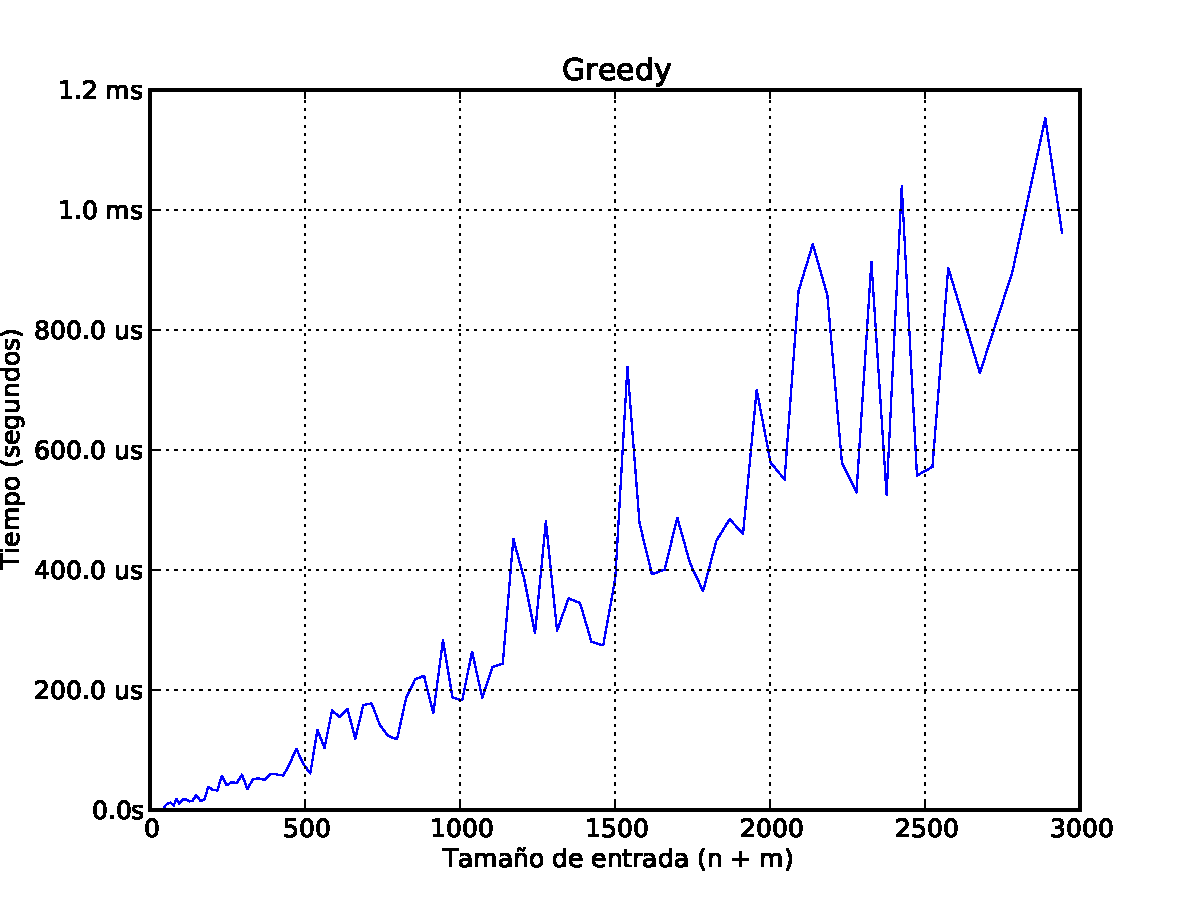
\includegraphics[angle=0, scale=.75]{imagenes/tiempos_greedy_magic/greedy_A_2014-06-27_02-37-46.pdf}
\label{grafico local}
\end{center}
\end{figure}

Se puede interpretar la curva de tiempo de ejecución vs. tamaño de entrada como una función cercana a la lineal, aunque se puede percibir
que está ligeramente por encima de ésta.

\begin{figure}[H]
\begin{center}
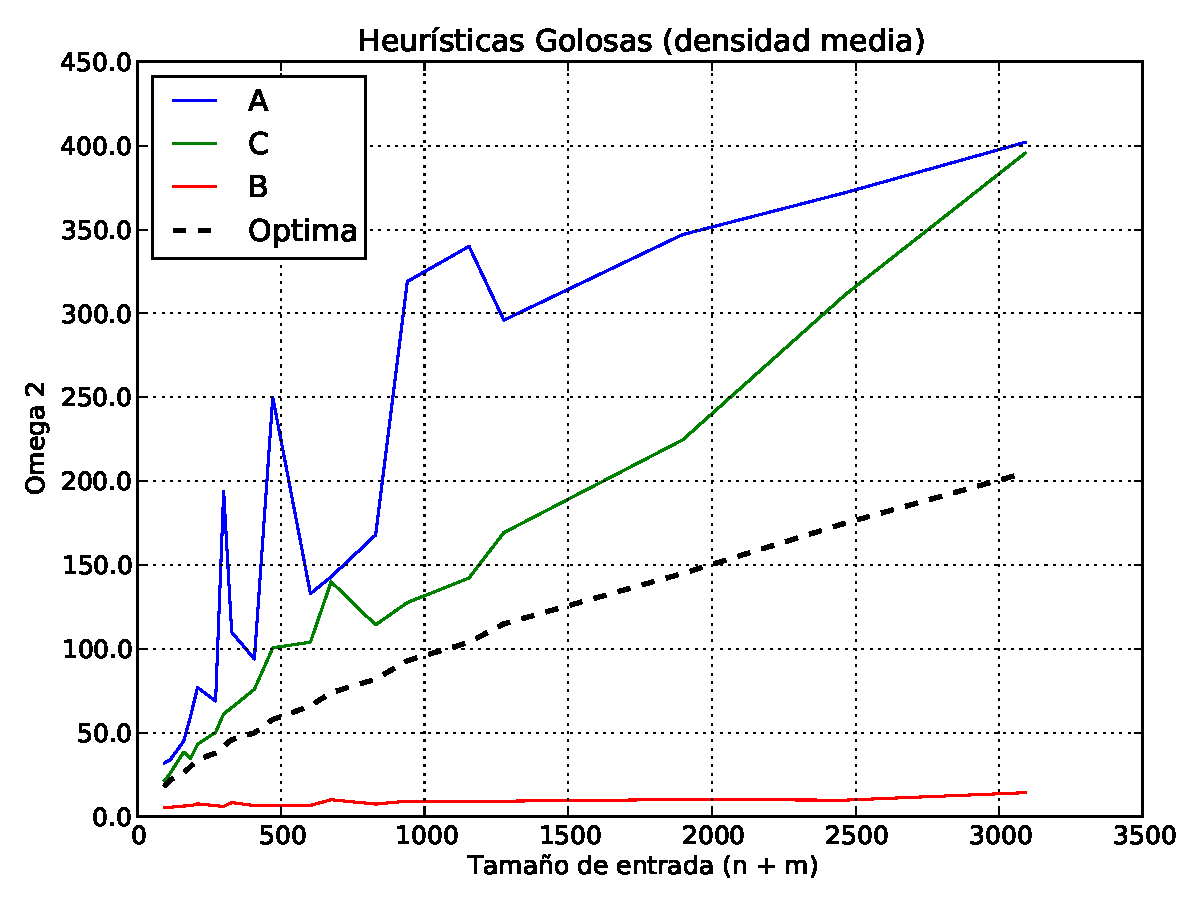
\includegraphics[angle=0, scale=.75]{imagenes/calidad_greedy_2014-06-27_09-50-48.pdf}
\label{grafico local}
\end{center}
\end{figure}

Lo que salta a simple vista es el bajo peso según $\omega_2$ de la heurística B. ¡Pareciera ser mejor solución que la óptima! Sin embargo,
recordando lo expuesto previamente, nos damos cuenta que si el peso según $\omega_2$ es menor que el de la óptima, entonces el peso según
$\omega_1$ es mayor que el de la óptima, es decir, que $k$. Por lo tanto no son soluciones válidas.
Ésto era de esperar - la heurística B sólo va construyendo su solución sin reparar siquiera en $\omega_1$.

Por otro lado tenemos la heurística A, que sólo mira $\omega_1$ y por lo tanto termina bastante alejada de la solución óptima. La heurística
C resultó ser un acierto, se acerca bastante a la solución válida, pero no descuida el mantenerse dentro de la cota de $k$.
